\documentclass[10pt,twocolumn]{article}
\usepackage[margin=0.75in]{geometry}
\usepackage[T1]{fontenc}
\usepackage{newtxtext,newtxmath}
\usepackage{microtype}
\usepackage{booktabs}
\usepackage{array}
\usepackage{graphicx}
\usepackage{xcolor}
\usepackage{url}
\usepackage[hidelinks]{hyperref}
\usepackage[numbers,sort]{natbib}
\usepackage{enumitem}
\setlist{nosep,leftmargin=*}
\usepackage[font=small,labelfont=bf]{caption}
\usepackage{xspace}

% Every number in this paper is a macro generated by paper/make_tables.py from benchmarks/results/paper_*.json.
% Generated by paper/make_tables.py from benchmarks/results/paper_*.json. Do not edit.
\newcommand{\AgentExposed}{5, 5, 5}
\newcommand{\AgentExposedFns}{clamp\_percent, clip\_negatives, count\_positive, dedupe\_sorted, normalize\_to\_unit}
\newcommand{\AgentFalseClaims}{0, 0, 0}
\newcommand{\AgentFalsificationMin}{1.5}
\newcommand{\AgentNewBeyond}{58, 66, 65}
\newcommand{\AgentNonvacRate}{1.00 (0.00)}
\newcommand{\AgentNotProposed}{0}
\newcommand{\AgentRawCands}{81, 89, 84}
\newcommand{\AgentRejectedWhole}{0}
\newcommand{\AgentRunOutcomes}{COMPLETE}
\newcommand{\AgentRuns}{3}
\newcommand{\AgentSchemaRate}{1.00 (0.00)}
\newcommand{\AgentTopRejections}{none}
\newcommand{\ConsCompared}{13{,}210}
\newcommand{\ConsCovLoss}{5{,}305}
\newcommand{\ConsFirstCompared}{13{,}210}
\newcommand{\ConsFirstMismatch}{0}
\newcommand{\ConsIntroFull}{2{,}164}
\newcommand{\ConsMismatch}{0}
\newcommand{\ConsMissed}{2{,}031}
\newcommand{\EngCombinedAbst}{3}
\newcommand{\EngCombinedFN}{0}
\newcommand{\EngCombinedFP}{0}
\newcommand{\EngCombinedTN}{1}
\newcommand{\EngCombinedTP}{5}
\newcommand{\EngDynamicAbst}{0}
\newcommand{\EngDynamicFN}{0}
\newcommand{\EngDynamicFP}{0}
\newcommand{\EngDynamicTN}{4}
\newcommand{\EngDynamicTP}{5}
\newcommand{\EngStaticAbst}{5}
\newcommand{\EngStaticFN}{3}
\newcommand{\EngStaticFP}{0}
\newcommand{\EngStaticTN}{1}
\newcommand{\EngStaticTP}{0}
\newcommand{\ExposedEveryAgentRun}{clamp\_percent, clip\_negatives, count\_positive, dedupe\_sorted, normalize\_to\_unit}
\newcommand{\ExposedEveryModelRun}{clip\_negatives, dedupe\_sorted}
\newcommand{\ExposedOnlyAgent}{clamp\_percent, count\_positive, normalize\_to\_unit}
\newcommand{\ExposedOnlyModel}{none}
\newcommand{\ExposedUnionBoth}{5}
\newcommand{\HostContainers}{10}
\newcommand{\HostCpu}{Apple M4}
\newcommand{\HostDocker}{29.5.2}
\newcommand{\HostEngine}{0.5.0}
\newcommand{\HostLoadMax}{137}
\newcommand{\HostLoadMedian}{7}
\newcommand{\HostLoadSamples}{208}
\newcommand{\HostLoadWindow}{2026-10-08 23:43 to 2026-10-09 03:26}
\newcommand{\HostModel}{Mac16,12}
\newcommand{\HostOllama}{0.40.1}
\newcommand{\HostOs}{macOS 15.6 (24G84)}
\newcommand{\HostPython}{3.13.9}
\newcommand{\HostRamGB}{16}
\newcommand{\HostSemantics}{python3.13-cpython-builtin-v4}
\newcommand{\HostSourceDigest}{451eaf54f534}
\newcommand{\HostSwapMaxGB}{18.5}
\newcommand{\HostSwapMedianGB}{13.0}
\newcommand{\HostZThree}{5.1.0}
\newcommand{\ImplSrcFiles}{68}
\newcommand{\ImplSrcLines}{17{,}617}
\newcommand{\ImplTestLines}{8{,}404}
\newcommand{\LatFirstFullIncomplete}{8}
\newcommand{\LatFirstFullRuns}{263}
\newcommand{\LatFirstLoadMax}{93.7}
\newcommand{\LatFirstLoadMedian}{7.2}
\newcommand{\LatFullUnresolvedMax}{5}
\newcommand{\LatFullUnresolvedMin}{1}
\newcommand{\LatHHubFullColdN}{30}
\newcommand{\LatHHubFullColdOutcome}{PASS}
\newcommand{\LatHHubFullColdPfifty}{1{,}450}
\newcommand{\LatHHubFullColdPninetyfive}{1{,}536}
\newcommand{\LatHHubFullColdRss}{81}
\newcommand{\LatHHubFullWarmN}{30}
\newcommand{\LatHHubFullWarmOutcome}{PASS}
\newcommand{\LatHHubFullWarmPfifty}{672}
\newcommand{\LatHHubFullWarmPninetyfive}{704}
\newcommand{\LatHHubFullWarmRss}{45}
\newcommand{\LatHHubQuickColdN}{30}
\newcommand{\LatHHubQuickColdOutcome}{PASS}
\newcommand{\LatHHubQuickColdPfifty}{855}
\newcommand{\LatHHubQuickColdPninetyfive}{916}
\newcommand{\LatHHubQuickColdRss}{66}
\newcommand{\LatHHubQuickWarmN}{30}
\newcommand{\LatHHubQuickWarmOutcome}{PASS}
\newcommand{\LatHHubQuickWarmPfifty}{563}
\newcommand{\LatHHubQuickWarmPninetyfive}{604}
\newcommand{\LatHHubQuickWarmRss}{42}
\newcommand{\LatHLeafFullColdN}{30}
\newcommand{\LatHLeafFullColdOutcome}{PASS}
\newcommand{\LatHLeafFullColdPfifty}{1{,}456}
\newcommand{\LatHLeafFullColdPninetyfive}{1{,}607}
\newcommand{\LatHLeafFullColdRss}{82}
\newcommand{\LatHLeafFullWarmN}{30}
\newcommand{\LatHLeafFullWarmOutcome}{PASS}
\newcommand{\LatHLeafFullWarmPfifty}{668}
\newcommand{\LatHLeafFullWarmPninetyfive}{690}
\newcommand{\LatHLeafFullWarmRss}{46}
\newcommand{\LatHLeafQuickColdN}{30}
\newcommand{\LatHLeafQuickColdOutcome}{PASS}
\newcommand{\LatHLeafQuickColdPfifty}{493}
\newcommand{\LatHLeafQuickColdPninetyfive}{517}
\newcommand{\LatHLeafQuickColdRss}{39}
\newcommand{\LatHLeafQuickWarmN}{30}
\newcommand{\LatHLeafQuickWarmOutcome}{PASS}
\newcommand{\LatHLeafQuickWarmPfifty}{496}
\newcommand{\LatHLeafQuickWarmPninetyfive}{598}
\newcommand{\LatHLeafQuickWarmRss}{40}
\newcommand{\LatKHubFullColdN}{30}
\newcommand{\LatKHubFullColdOutcome}{PASS}
\newcommand{\LatKHubFullColdPfifty}{9{,}930}
\newcommand{\LatKHubFullColdPninetyfive}{15{,}753}
\newcommand{\LatKHubFullColdRss}{173}
\newcommand{\LatKHubFullWarmN}{30}
\newcommand{\LatKHubFullWarmOutcome}{PASS}
\newcommand{\LatKHubFullWarmPfifty}{3{,}578}
\newcommand{\LatKHubFullWarmPninetyfive}{4{,}293}
\newcommand{\LatKHubFullWarmRss}{152}
\newcommand{\LatKHubQuickColdN}{30}
\newcommand{\LatKHubQuickColdOutcome}{INCOMPLETE}
\newcommand{\LatKHubQuickColdPfifty}{4{,}483}
\newcommand{\LatKHubQuickColdPninetyfive}{4{,}711}
\newcommand{\LatKHubQuickColdRss}{135}
\newcommand{\LatKHubQuickWarmN}{30}
\newcommand{\LatKHubQuickWarmOutcome}{PASS}
\newcommand{\LatKHubQuickWarmPfifty}{2{,}401}
\newcommand{\LatKHubQuickWarmPninetyfive}{2{,}741}
\newcommand{\LatKHubQuickWarmRss}{118}
\newcommand{\LatKLeafFullColdN}{30}
\newcommand{\LatKLeafFullColdOutcome}{PASS}
\newcommand{\LatKLeafFullColdPfifty}{9{,}334}
\newcommand{\LatKLeafFullColdPninetyfive}{13{,}711}
\newcommand{\LatKLeafFullColdRss}{180}
\newcommand{\LatKLeafFullWarmN}{30}
\newcommand{\LatKLeafFullWarmOutcome}{PASS}
\newcommand{\LatKLeafFullWarmPfifty}{3{,}388}
\newcommand{\LatKLeafFullWarmPninetyfive}{3{,}599}
\newcommand{\LatKLeafFullWarmRss}{152}
\newcommand{\LatKLeafQuickColdN}{30}
\newcommand{\LatKLeafQuickColdOutcome}{PASS}
\newcommand{\LatKLeafQuickColdPfifty}{1{,}445}
\newcommand{\LatKLeafQuickColdPninetyfive}{1{,}488}
\newcommand{\LatKLeafQuickColdRss}{84}
\newcommand{\LatKLeafQuickWarmN}{30}
\newcommand{\LatKLeafQuickWarmOutcome}{PASS}
\newcommand{\LatKLeafQuickWarmPfifty}{1{,}435}
\newcommand{\LatKLeafQuickWarmPninetyfive}{1{,}495}
\newcommand{\LatKLeafQuickWarmRss}{84}
\newcommand{\LatLoadMax}{10.4}
\newcommand{\LatLoadMedian}{3.9}
\newcommand{\LatLoadMin}{2.0}
\newcommand{\LatMaxRss}{756}
\newcommand{\LatRatioMax}{4.16}
\newcommand{\LatRatioMedian}{1.07}
\newcommand{\LatRatioMin}{0.87}
\newcommand{\LatRepeatFullIncomplete}{2}
\newcommand{\LatRepeatFullRuns}{263}
\newcommand{\LatReps}{30}
\newcommand{\LatRepsLarge}{5}
\newcommand{\LatSwapFirstMax}{11.9}
\newcommand{\LatSwapFirstMin}{8.9}
\newcommand{\LatSwapFirstSamples}{62}
\newcommand{\LatSwapRepeatMax}{15.4}
\newcommand{\LatSwapRepeatMin}{11.9}
\newcommand{\LatSwapRepeatSamples}{65}
\newcommand{\LatTKHubFullColdN}{5}
\newcommand{\LatTKHubFullColdOutcome}{PASS}
\newcommand{\LatTKHubFullColdPfifty}{129{,}902}
\newcommand{\LatTKHubFullColdPninetyfive}{135{,}368}
\newcommand{\LatTKHubFullColdRss}{565}
\newcommand{\LatTKHubFullWarmN}{5}
\newcommand{\LatTKHubFullWarmOutcome}{PASS}
\newcommand{\LatTKHubFullWarmPfifty}{35{,}696}
\newcommand{\LatTKHubFullWarmPninetyfive}{42{,}447}
\newcommand{\LatTKHubFullWarmRss}{698}
\newcommand{\LatTKHubQuickColdN}{5}
\newcommand{\LatTKHubQuickColdOutcome}{INCOMPLETE}
\newcommand{\LatTKHubQuickColdPfifty}{39{,}896}
\newcommand{\LatTKHubQuickColdPninetyfive}{45{,}567}
\newcommand{\LatTKHubQuickColdRss}{492}
\newcommand{\LatTKHubQuickWarmN}{5}
\newcommand{\LatTKHubQuickWarmOutcome}{INCOMPLETE}
\newcommand{\LatTKHubQuickWarmPfifty}{32{,}328}
\newcommand{\LatTKHubQuickWarmPninetyfive}{33{,}837}
\newcommand{\LatTKHubQuickWarmRss}{514}
\newcommand{\LatTKLeafFullColdN}{5}
\newcommand{\LatTKLeafFullColdOutcome}{INCOMPLETE (2); PASS (3)}
\newcommand{\LatTKLeafFullColdPfifty}{116{,}354}
\newcommand{\LatTKLeafFullColdPninetyfive}{124{,}784}
\newcommand{\LatTKLeafFullColdRss}{549}
\newcommand{\LatTKLeafFullWarmN}{5}
\newcommand{\LatTKLeafFullWarmOutcome}{PASS}
\newcommand{\LatTKLeafFullWarmPfifty}{42{,}714}
\newcommand{\LatTKLeafFullWarmPninetyfive}{54{,}785}
\newcommand{\LatTKLeafFullWarmRss}{599}
\newcommand{\LatTKLeafQuickColdN}{5}
\newcommand{\LatTKLeafQuickColdOutcome}{PASS}
\newcommand{\LatTKLeafQuickColdPfifty}{14{,}335}
\newcommand{\LatTKLeafQuickColdPninetyfive}{17{,}925}
\newcommand{\LatTKLeafQuickColdRss}{380}
\newcommand{\LatTKLeafQuickWarmN}{5}
\newcommand{\LatTKLeafQuickWarmOutcome}{PASS}
\newcommand{\LatTKLeafQuickWarmPfifty}{13{,}961}
\newcommand{\LatTKLeafQuickWarmPninetyfive}{14{,}307}
\newcommand{\LatTKLeafQuickWarmRss}{375}
\newcommand{\ModelAttempted}{39}
\newcommand{\ModelCalls}{39}
\newcommand{\ModelDistinctResponseSets}{3}
\newcommand{\ModelExposed}{2, 2, 2}
\newcommand{\ModelExposedFns}{clip\_negatives, dedupe\_sorted}
\newcommand{\ModelFalseClaims}{8, 6, 8}
\newcommand{\ModelFunctions}{13}
\newcommand{\ModelIdentical}{no}
\newcommand{\ModelLatMax}{145.8}
\newcommand{\ModelLatMin}{28.7}
\newcommand{\ModelLatPfifty}{92.2}
\newcommand{\ModelLatPninetyfive}{128.4}
\newcommand{\ModelNewBeyond}{11, 9, 12}
\newcommand{\ModelNonvacRate}{0.66 (0.03)}
\newcommand{\ModelRawCands}{35, 35, 35}
\newcommand{\ModelRepeats}{3}
\newcommand{\ModelRss}{4{,}918}
\newcommand{\ModelSeeded}{5}
\newcommand{\ModelTokPerS}{6.2}
\newcommand{\ModelTopRejections}{TYPE\_ERROR (22), VACUOUS\_PREDICATE (8), DUPLICATE (6)}
\newcommand{\ModelWallMin}{20}
\newcommand{\RunDates}{2026-10-08, 2026-10-09}
\newcommand{\SeedAbstNegCases}{I01, N06, U03, P01, P02}
\newcommand{\SeedAbstPosCases}{U01, U04}
\newcommand{\SeedBestAbst}{0.21}
\newcommand{\SeedBestAbstNeg}{5}
\newcommand{\SeedBestAbstPos}{2}
\newcommand{\SeedBestFN}{1}
\newcommand{\SeedBestFP}{0}
\newcommand{\SeedBestPrec}{1.00}
\newcommand{\SeedBestRecA}{0.86}
\newcommand{\SeedBestRecD}{0.95}
\newcommand{\SeedBestTN}{7}
\newcommand{\SeedBestTP}{18}
\newcommand{\SeedBlocksOnNegatives}{0}
\newcommand{\SeedCases}{35}
\newcommand{\SeedContractCases}{11}
\newcommand{\SeedDisagree}{0}
\newcommand{\SeedDynamicMedianMs}{3{,}110}
\newcommand{\SeedExecCases}{11}
\newcommand{\SeedExecWallMedian}{4{,}639}
\newcommand{\SeedFalseNegCases}{U02}
\newcommand{\SeedFullWallMedian}{412}
\newcommand{\SeedIncCompared}{30}
\newcommand{\SeedIncMismatch}{0}
\newcommand{\SeedIncVerdictMismatch}{U02}
\newcommand{\SeedIncVerdictMismatchN}{1}
\newcommand{\SeedIntentBlocked}{I04}
\newcommand{\SeedIntentNotBlocked}{I01, I02, I03}
\newcommand{\SeedIntentional}{2}
\newcommand{\SeedLabelsFrozen}{2026-10-08T17:44:28Z}
\newcommand{\SeedManifestDigest}{94f276b0810d}
\newcommand{\SeedNeg}{12}
\newcommand{\SeedNegIncomplete}{5}
\newcommand{\SeedNegIncompleteCases}{I01, N06, U03, P01, P02}
\newcommand{\SeedPos}{21}
\newcommand{\SeedQuickAbstNeg}{5}
\newcommand{\SeedQuickAbstPos}{4}
\newcommand{\SeedQuickFN}{4}
\newcommand{\SeedQuickFP}{0}
\newcommand{\SeedQuickPrec}{1.00}
\newcommand{\SeedQuickRecA}{0.62}
\newcommand{\SeedQuickRecD}{0.76}
\newcommand{\SeedQuickTN}{7}
\newcommand{\SeedQuickTP}{13}
\newcommand{\SeedQuickWallMedian}{408}
\newcommand{\SeedRunnerProbeMedianMs}{955}
\newcommand{\SeedSolverChanged}{0}
\newcommand{\SeedSolverCompared}{30}
\newcommand{\SeedSolverVerdictChanged}{0}
\newcommand{\SeedWarmCompared}{30}
\newcommand{\SeedWarmMismatch}{0}
\newcommand{\SeedWarnFlags}{S04, S07}
\newcommand{\SeededDslExpressible}{5}
\newcommand{\SemAbstRate}{0.32}
\newcommand{\SemAbstainNeg}{1}
\newcommand{\SemAbstainPos}{8}
\newcommand{\SemCases}{31}
\newcommand{\SemConfirmed}{28}
\newcommand{\SemFN}{0}
\newcommand{\SemFP}{0}
\newcommand{\SemIndeterminate}{3}
\newcommand{\SemLabeled}{28}
\newcommand{\SemMatch}{31}
\newcommand{\SemMatchNoSolver}{31}
\newcommand{\SemNeg}{10}
\newcommand{\SemNoSolverAbst}{10}
\newcommand{\SemNoSolverTN}{8}
\newcommand{\SemNoSolverTP}{10}
\newcommand{\SemPos}{18}
\newcommand{\SemPrecision}{1.00}
\newcommand{\SemRecallA}{0.56}
\newcommand{\SemRecallD}{1.00}
\newcommand{\SemSolverChanged}{2}
\newcommand{\SemSolverChangedList}{two-variable-equality, unknown-call-unrelated}
\newcommand{\SemTN}{9}
\newcommand{\SemTP}{10}
\newcommand{\SemUnlabeled}{3}
\newcommand{\TemplateExposed}{0, 0, 0}
\newcommand{\TemplateRawCands}{23, 23, 23}
\newcommand{\TemplateRefuted}{0, 0, 0}
\newcommand{\TemplateTested}{23, 23, 23}
\newcommand{\TestSeconds}{206}
\newcommand{\TestSummary}{788 passed, 2 skipped, 1 xfailed}
\newcommand{\TransportAnswered}{13}
\newcommand{\TransportExposed}{3}
\newcommand{\TransportFunctions}{13}
\newcommand{\TransportLatPfifty}{73.4}
\newcommand{\TransportLeft}{no}
\newcommand{\TransportNonvac}{24}
\newcommand{\TransportRaw}{35}
\newcommand{\TransportSchemaRate}{0.83}
\newcommand{\TransportServed}{qwen2.5-coder:7b}
\newcommand{\TransportStatus}{AVAILABLE}
\newcommand{\TransportStructured}{json\_schema (13)}
\newcommand{\TransportWallMin}{16}

\newcommand{\opt}[1]{\texttt{-{}-#1}}
\newcommand{\res}[1]{\texttt{\small #1}}

\title{Keeping Proof, Execution and Authority Apart When Verifying Coding-Agent Patches:\\
An Empirical Report on a Local-First Prototype}
\author{InvariantGuard repository authors\thanks{Disclosure: the prototype, its benchmarks and this report were produced by
AI coding agents (Claude Opus 5.5) in a human-directed, specification-driven workflow. The agent-proposed contracts evaluated in
Section~\ref{sec:rq5} come from Claude Sonnet 5.5, a model of the same family. See Section~\ref{sec:threats}.}\\
{\small Workshop draft. Every number is generated from \texttt{benchmarks/results/paper\_*.json}; see \texttt{paper/README.md}.}}
\date{}

\begin{document}
\maketitle

\begin{abstract}
Coding agents need machine-checkable feedback on the patches they write. A single pass/fail or ``confidence'' signal
mixes up different kinds of evidence: a proof under stated assumptions, a finite test, an observed regression, and an
inferred property that nobody approved. We describe InvariantGuard, a local-first prototype that checks a patch
against an explicit base snapshot with two engines. A static engine handles modeled runtime failures (zero divisors,
sequence bounds, \texttt{None} attribute access) over a small typed IR for a Python subset. A contract engine replays
typed behavioral properties on the base and the patch inside an isolated container. Proposers (templates, a local
open-weight model, or the calling coding agent) may suggest contracts, but they never decide whether a contract holds
or how much authority it has. Every result keeps proof status, scope, authority, patch relation, coverage and the gate
verdict on separate axes. Unsupported code is reported as \res{UNKNOWN}/\res{INCOMPLETE} rather than dropped. We
evaluate the implementation on \SemCases{} controlled fixtures, on \SeedCases{} hand-written baseline/patch pairs whose
labels were frozen before any tool run, with ablations, with latency on synthetic repositories of about 100 to
10{,}000 functions, and with three contract proposers on \ModelFunctions{} held-out functions. On execution-confirmed seeded labels,
the best configuration flagged \SeedBestTP{} of \SeedPos{} introduced defects, abstained on \SeedBestAbstPos{} and
missed \SeedBestFN{}, with \SeedBestFP{} false positives on \SeedNeg{} negatives. It abstained on \SeedBestAbstNeg{} of
those negatives. The single miss exposed a quick-mode slicing defect in the prototype. Blinded agent-proposed contracts
exposed more seeded bugs than the local model (per run: \AgentExposed{} versus \ModelExposed{} of \ModelSeeded{}).
That comparison is confounded by the prompt, the candidate cap, model scale, and model-family overlap with the benchmark author. All
benchmarks are synthetic or author-written and ran on one machine. They do not establish effectiveness on natural agent
patches.
\end{abstract}

\section{Introduction}

Coding agents increasingly propose patches that a person or another agent must accept or reject. Tests, type checkers
and a reviewer's reading each give a different kind of evidence. When a tool reports on a patch, the consumer (often
another model) needs to know \emph{what} was established, under \emph{which} assumptions and for \emph{which} inputs.
It also needs to know whether the claim is about the patch or about code that was already there.

This report describes InvariantGuard, a prototype built to explore that question, and evaluates it empirically. The
prototype is deliberately narrow: a Python subset, three static properties, a small typed property language for
contracts, and an isolated runner for differential replay. Our contributions are modest and empirical:
\begin{itemize}
\item We frame verification results as \emph{evidence axes} that keep proof status, scope validity, authority, patch
  relation, coverage, run outcome and verdict separate. We use this framing to organize a whole tool
  (Section~\ref{sec:framing}).
\item We built a working, local-first implementation. It combines change-scoped static checking, base-versus-patch
  contract replay, and contract proposers that can only suggest. The proposers are templates, a local model reached only
  over loopback, and the calling agent through a context-packet protocol
  (Sections~\ref{sec:design}--\ref{sec:impl}).
\item We give a reproducible evaluation. It reports explicit denominators, keeps abstentions in every rate, freezes
  labels before tool runs, and discloses a defect that the evaluation found in the prototype (Section~\ref{sec:eval}).
\end{itemize}
We do not claim that any component is new. Static runtime-error detection, dynamic invariant discovery, SMT-based
checking and agent-driven property-based testing are all established (Section~\ref{sec:related}).

\section{Problem framing: evidence axes}
\label{sec:framing}

A verification result for a patch answers several independent questions. Collapsing them into one number hides exactly
the information that an agent needs to repair a patch, or that a person needs to accept it. InvariantGuard attaches
the following axes to every obligation and contract result:

\smallskip\noindent{\small\begin{tabular}{@{}>{\raggedright\arraybackslash}p{0.22\columnwidth}>{\raggedright\arraybackslash}p{0.73\columnwidth}@{}}
\toprule
axis & values \\
\midrule
property result & \res{PROVED\_SAFE}, \res{PROVED\_UNSAFE}, \res{POSSIBLY\_UNSAFE}, \res{TESTED}, \res{OBSERVED\_FAILURE}, \res{OBSERVED\_REGRESSION}, \res{UNVERIFIED}, \res{UNKNOWN}\\
scope validity & \res{EXACT\_MODEL}, \res{CONDITIONAL}, \res{OVERAPPROXIMATE}, \res{BOUNDED}, \res{EXECUTED}\\
authority & \res{DECLARED}, \res{APPROVED}, \res{INFERRED}, \res{REJECTED}, \res{RETIRED}\\
patch relation & \res{INTRODUCED}, \res{PRE\_EXISTING}, \res{RESOLVED}, \res{CHANGED}, \res{UNDETERMINED}\\
run outcome & \res{COMPLETE}, \res{INCOMPLETE}, \res{ERROR}, \res{CANCELLED}\\
verdict & \res{PASS}, \res{WARN}, \res{BLOCK}, \res{INCOMPLETE}, \res{ERROR}\\
\bottomrule
\end{tabular}}
\smallskip

The axes encode distinctions that are easy to lose. A satisfiable query over an exact model of the admitted inputs
yields \res{PROVED\_UNSAFE} with a concrete witness. The same query over an overapproximation yields only
\res{POSSIBLY\_UNSAFE}. Python does not enforce type annotations at runtime, so a result that relies on them is
\res{CONDITIONAL}, not \res{EXACT\_MODEL}. Passing probes give \res{TESTED}, a finite claim, never a proof. A result is
an \res{OBSERVED\_REGRESSION} only when the same admitted input satisfies the property on the base and violates it on
the patch, in comparable environments. If both versions fail, the relation is \res{PRE\_EXISTING}. Authority records
who stands behind a property. A contract inferred from old behavior (\res{INFERRED}) is not evidence of intent, so it
can only warn.

The gate verdict is a policy over the axes, with precedence \res{ERROR} $>$ \res{BLOCK} $>$ \res{INCOMPLETE} $>$
\res{WARN} $>$ \res{PASS}. Two cases block: an introduced exact failure under a declared domain, and a replayed
regression of a declared or approved contract. Conditional or overapproximate failures warn, and so do changes to
inferred contracts. Some required obligations can remain \res{UNKNOWN}: unsupported constructs, solver timeouts,
exhausted budgets and unavailable runners all cause this. They make the run \res{INCOMPLETE}, which is never reported as
\res{PASS}. Required coverage is fixed in the analysis plan before analysis starts.

\section{Design}
\label{sec:design}

\paragraph{Typed IR and semantic profiles.}
The Python frontend parses source with the standard \texttt{ast} and \texttt{symtable} modules. It never imports or
executes the repository. Supported module-level functions are lowered to a small typed CFG IR: constants, parameters,
integer arithmetic, the three division operators, comparisons, \texttt{is None}, \texttt{len}, indexing, calls,
attributes, branches, $\phi$-joins, and an explicit \texttt{UNKNOWN\_EFFECT}. Each operation carries a semantic profile
rather than a generic meaning~\cite{python_expressions}. Python \texttt{//} and \texttt{\%} use floor semantics,
integers are unbounded, and negative indices are valid in $[-n, n)$. Assertions are lowered with
\texttt{\_\_debug\_\_} as an explicit runtime-mode input, so behavior under \texttt{python -O} is modeled. Some operands
are not established exact built-ins, for example a value returned by an unmodeled call, which may dispatch to a
user-defined operator. Such operands make the dependent obligation \res{UNKNOWN}, or \res{CONDITIONAL} when only an
annotation supports the type. Loops, nested functions, methods, comprehensions, lambdas, decorators and exception
handlers are outside the subset. Their obligations are reported as \res{UNKNOWN} with a reason and stay in the
denominator.

\paragraph{Static decision procedure.}
An obligation is a syntactic division, a subscript of an established list or tuple, or an attribute load on a value
that may be \texttt{None}. The engine first applies unsupported-region checks and reachability. It then tries cheap
interval and path facts, and finally, optionally, an SMT query \emph{path condition $\wedge$ bad state} in
Z3~\cite{demoura2008z3}. \texttt{UNSAT} gives \res{PROVED\_SAFE}. A \texttt{SAT} model is re-validated by a concrete IR
evaluator before it becomes a \res{PROVED\_UNSAFE} witness. Without the solver, a deterministic bounded witness search
remains. A call to a supported function in the same snapshot is instantiated at the call site. Resolving a call across
modules makes the result \res{CONDITIONAL} on import resolution.

\paragraph{Change-scoped verification.}
\texttt{guard verify -{}-base REF} captures immutable, content-addressed snapshots of two trees: the base (a Git commit or
a saved baseline) and the working tree, including uncommitted changes. It aborts or restarts if files change during
capture. Symbols are matched across the two snapshots. A dependency graph over calls, imports, global reads and contract
scopes seeds an affected slice from the changed symbols. Per-symbol validity keys gate cache reuse; they cover the
normalized IR, transitive dependencies, configuration, semantic profile, solver and contract digests. \emph{Quick} mode
analyzes the affected slice within a budget (default 2\,s) and reports \res{INCOMPLETE} if the budget runs out.
\emph{Full} mode analyzes the whole scope. Each failure in the candidate is matched to a base obligation, and its
witness is replayed against the base model. The result is \res{INTRODUCED}, \res{PRE\_EXISTING} or \res{RESOLVED}. When
attribution is impossible the relation is \res{UNDETERMINED}; attribution is required work, so the run is
\res{INCOMPLETE}.

\paragraph{Contracts and authority.}
A behavioral contract is a typed JSON predicate in a small DSL. The DSL has references to arguments, results and
before/after argument snapshots; comparisons; boolean connectives; \texttt{len}; \texttt{sum}; \texttt{approx\_eq} with
mandatory tolerances; \texttt{all\_between}; \texttt{unchanged\_argument}; and \texttt{repeatability}. There is no
indexing and no arithmetic, and candidate strings are never evaluated. Each contract has an input profile (bounded
built-in values), a precondition, an authority, and an append-only history of revisions and evidence. With
\opt{execute}, admitted inputs run on \emph{both} snapshots in a Docker container. The container has no network,
read-only source, dropped capabilities and resource limits, and the runner checks these from inside before any import.
The predicate is evaluated on the host over an exact encoding of built-in values. Counterexamples are shrunk within the
domain and confirmed in fresh runs. An intentional API change is accepted through an auditable contract revision, never
by deleting evidence.

\paragraph{Proposers, not judges.}
Contract discovery has five sources. All of them share one parser and one validation pipeline: typed DSL, symbols,
budgets, an admissible precondition, a behavioral non-vacuity filter, de-duplication, and optional isolated
falsification. Every accepted candidate is recorded as \res{INFERRED} at most.
\begin{itemize}
\item \emph{Templates}: purity, length preservation, assertions and repeatability.
\item \emph{A local open-weight model}: reached only over a validated loopback endpoint, pinned by digest, never
  downloaded during a scan.
\item \emph{Bring-your-own-key adapters} for OpenAI-compatible and Anthropic endpoints: opt-in, with https and explicit
  permission required for any non-loopback host. Each data egress is recorded per function. There is no fallback in
  either direction.
\item \emph{The calling coding agent}: it reads a \emph{context packet} (MCP \texttt{get\_context\_packet} or
  \texttt{guard contracts context}) and submits a batch bound to the packet's digest. A batch for a different packet is
  rejected as stale. The batch schema has no field for authority, approval or evidence, and the proposer's identity is
  taken from the transport and labeled as self-reported.
\end{itemize}
The context packet is AST-only and budgeted (12{,}000 bytes), and it frames all source as untrusted data. It is the same
object for the local model and for the agent. Model and agent output never becomes a proof assumption, and no tool can
approve a contract.

\paragraph{Agent interface.}
All commands emit schema-validated JSON with stable finding identifiers, witnesses, source spans and explicit coverage.
A stdio Model Context Protocol server~\cite{mcp2025transports,mcp_python_sdk} exposes verification, evidence retrieval
and contract proposal over the same orchestration code as the CLI. It has no tool that approves contracts, changes
baselines or executes commands.

\section{Implementation}
\label{sec:impl}

The prototype is \ImplSrcLines{} lines of Python in \ImplSrcFiles{} files (engine \HostEngine{}, semantics profile
\texttt{\HostSemantics}). The core uses only the standard library. Z3 \HostZThree{} is an optional solver dependency,
and the MCP SDK is an optional extra. On the evaluation host the test suite (\ImplTestLines{} lines) reported
\emph{\TestSummary} in \TestSeconds\,s. The skips are opt-in tests against the real model, and the expected failure
records the defect discussed in Section~\ref{sec:rq4}. Contract checks use Docker \HostDocker{} with a pinned
\texttt{python:3.13-slim} image. The local model is \texttt{qwen2.5-coder:7b} (Q4\_K\_M, pinned by
digest)~\cite{hui2024qwen25coder}, served by Ollama \HostOllama{}. Dependencies are pinned in a lock file that equals
the environment's \texttt{pip freeze}.

\section{Evaluation}
\label{sec:eval}

\paragraph{Setup.}
All runs used one machine: \HostModel{} (\HostCpu{}, \HostRamGB\,GB RAM), \HostOs{}, CPython \HostPython{}, on
\RunDates{} (UTC). The host also ran unrelated applications. Among them were containers of another project, which Docker
Desktop restarted when it was launched for our runner. Sampled once a minute from \HostLoadWindow{} UTC (\HostLoadSamples{}
samples), the 1-minute load average had a median of \HostLoadMedian{} and a maximum of \HostLoadMax{} on 10 logical
CPUs, and up to \HostSwapMaxGB\,GB of swap was in use. Timings are therefore noisy (see RQ4).
\texttt{benchmarks/run\_all.py} produces every number below, and \texttt{paper/make\_tables.py} typesets them. We address
the research questions of the project's specification (\texttt{docs/12} in the repository) only as far as the data
allows.
\begin{itemize}
\item \textbf{RQ1}: How faithful is the static engine on controlled semantics, and how often does it abstain?
\item \textbf{RQ2}: How does change-aware verification behave on seeded patches, including safe, pre-existing and
  intentional changes? Does differential evidence avoid false blocks?
\item \textbf{RQ3}: How often does combining static and dynamic checking improve actionable findings?
\item \textbf{RQ4}: Does conservative change-aware (quick) verification agree with full verification, and what does it
  cost?
\item \textbf{RQ5}: Do mechanically checked proposer candidates (templates, a local model, a coding agent) add
  properties that expose bugs?
\end{itemize}
The last specified question, ``what does honest abstention cost?'', runs through all five.

\paragraph{Ground truth.}
Labels never come from the tool. For a \emph{defect} label, we executed a hand-written witness (for patches, on both
versions) in a separate \texttt{python -I} process and observed the failure. For a \emph{safe} label, we wrote a hand
argument and corroborated it, without proving it, on a finite input grid. Cases whose truth depends on code outside
the fixture are unlabeled and excluded from precision and recall, but they are still counted. Abstentions (\res{UNKNOWN},
\res{INCOMPLETE}) remain in all denominators. We report recall two ways: with abstentions counted as misses
(Rec.\textsubscript{a}), and over decided cases only (Rec.\textsubscript{d}).

\subsection{RQ1: controlled semantic fixtures}

The \SemCases{} controlled fixtures exercise one obligation each. They cover guarded and unguarded division, infeasible
branches, relational guards, annotation-only domains, floor semantics, assertion runtime mode, empty lists, negative
indices, \texttt{None} flow and a changed callee. They also cover unsupported constructs: loops, methods, decorators,
closures, unknown calls, floats, \texttt{isinstance} with \texttt{bool}, and a nonlinear query whose smallest known
solution has 16-digit coordinates. \SemLabeled{} cases have an independent label (\SemPos{} defects, \SemNeg{} safe);
\SemIndeterminate{} do not. All \SemCases{} results matched the specified expectation, with and without the solver
(Table~\ref{tab:semantic}).

With the solver, the engine raised no false alarm (\SemFP{} FP) and missed no defect that it decided (\SemFN{} FN).
However, it abstained on \SemAbstainPos{} of the \SemPos{} defects and on \SemAbstainNeg{} safe case, so
Rec.\textsubscript{a} is \SemRecallA{} while Rec.\textsubscript{d} is \SemRecallD{}. The abstentions are the documented
subset boundary (loops, methods, decorators, closures, floats, \texttt{isinstance}, list element values, aliasing,
unknown callees) plus a solver timeout. Disabling the solver changed \SemSolverChanged{} result(s): \SemSolverChangedList.
Intervals cannot prove the relational guard $a \ne b \Rightarrow a-b \ne 0$, so that obligation becomes \res{UNKNOWN}.
The \res{POSSIBLY\_UNSAFE} result on an overapproximated path also becomes \res{UNKNOWN}. These fixtures were written
during development and serve as regression tests. They therefore measure conformance to the specification, not
generalization.

\begin{table*}[t]
\centering
\small

\caption{Controlled semantic fixtures (one obligation per case). Result counts over all cases; ``=spec'' is agreement with the specified expected result; the confusion counts use only cases with an independent label (defect: witness executed; safe: hand argument plus finite grid). Rec.\textsubscript{a} counts abstentions as misses; Rec.\textsubscript{d} uses decided cases only.}
\label{tab:semantic}
\begin{tabular}{lrrrrrrrrrrrrrr}
\toprule
 & SAFE & UNSAFE & POSS. & UNK. & =spec & TP & FP & FN & TN & Abst. & Prec. & Rec.\textsubscript{a} & Rec.\textsubscript{d} & Abst.\,rate \\
\midrule
solver on & 9 & 10 & 1 & 11 & 31/31 & 10 & 0 & 0 & 9 & 9 & 1.00 & 0.56 & 1.00 & 0.32 \\
solver off & 8 & 10 & 0 & 13 & 31/31 & 10 & 0 & 0 & 8 & 10 & 1.00 & 0.56 & 1.00 & 0.36 \\
\bottomrule
\end{tabular}
\end{table*}


\subsection{RQ2: seeded baseline/patch pairs}
\label{sec:rq2}

We wrote \SeedCases{} small baseline/patch pairs for this evaluation. They cover nine classes:
\begin{itemize}
\item removed, weakened or reordered division guards;
\item changed callees and constants that make unchanged callers unsafe;
\item off-by-one indices and removed emptiness guards;
\item \texttt{None} introduced directly or through a callee;
\item contract regressions (normalization, purity, length, range);
\item intentional changes, with and without a contract revision;
\item safe refactors;
\item cases outside the supported subset;
\item pre-existing failures.
\end{itemize}
Labels, oracle inputs and our a-priori expectation of the tool's outcome were frozen at \SeedLabelsFrozen{} (manifest
digest \texttt{\SeedManifestDigest\ldots}), before any tool run on these cases. Execution disagreed with
\SeedDisagree{} labels. Each case runs in a throwaway Git repository through the real CLI, with the patch left as
uncommitted changes. Table~\ref{tab:seeded-classes} gives the counts per class; the appendix lists every case.

\begin{table*}[t]
\centering
\small

\caption{Seeded patches by class. Left block: static quick verification (\texttt{guard verify -{}-mode quick}); right block: the best available configuration (the \texttt{-{}-execute} run for cases with contracts, otherwise static quick). A = abstained (required coverage missing: verdict INCOMPLETE without a flagged finding), kept in every denominator. The two \emph{intentional} labels are excluded from the counts and discussed in the text. Labels confirmed by executing both versions in a separate interpreter.}
\label{tab:seeded-classes}
\begin{tabular}{lrlrrrrrrrrrr}
\toprule
 & & & \multicolumn{5}{c}{static quick} & \multicolumn{5}{c}{best available} \\ \cmidrule(lr){4-8}\cmidrule(lr){9-13}
class & n & labels & TP & FN & A & FP & TN & TP & FN & A & FP & TN \\
\midrule
division by zero & 6 & 6 defect & 6 & 0 & 0 & 0 & 0 & 6 & 0 & 0 & 0 & 0 \\
changed callee & 2 & 2 defect & 2 & 0 & 0 & 0 & 0 & 2 & 0 & 0 & 0 & 0 \\
index bounds & 3 & 3 defect & 3 & 0 & 0 & 0 & 0 & 3 & 0 & 0 & 0 & 0 \\
None flow & 2 & 2 defect & 2 & 0 & 0 & 0 & 0 & 2 & 0 & 0 & 0 & 0 \\
contract regression & 5 & 5 defect & 0 & 3 & 2 & 0 & 0 & 5 & 0 & 0 & 0 & 0 \\
unsupported construct & 4 & 3 defect, 1 none & 0 & 1 & 3 & 0 & 0 & 0 & 1 & 3 & 0 & 0 \\
safe refactor & 7 & 7 none & 0 & 0 & 1 & 0 & 6 & 0 & 0 & 1 & 0 & 6 \\
intentional change & 4 & 2 intent., 2 none & 0 & 0 & 1 & 0 & 1 & 0 & 0 & 1 & 0 & 1 \\
pre-existing failure & 2 & 2 none & 0 & 0 & 2 & 0 & 0 & 0 & 0 & 2 & 0 & 0 \\
\midrule
all & 35 & 21 defect, 12 none, 2 intent. & 13 & 4 & 9 & 0 & 7 & 18 & 1 & 7 & 0 & 7 \\
\bottomrule
\end{tabular}
\end{table*}


Over the \SeedPos{} defect and \SeedNeg{} non-defect labels (Table~\ref{tab:seeded-confusion}), static quick
verification flagged \SeedQuickTP{} defects, abstained on \SeedQuickAbstPos{} and cleared \SeedQuickFN{}, with
\SeedQuickFP{} false positives. Three of the cleared defects are contract regressions that have no static obligation at
all. The static engine is \emph{correct} about its own properties there, but it cannot see the behavior the label is
about. The best configuration adds contract replay (\opt{execute}) for cases with contracts. It flagged \SeedBestTP{} of
\SeedPos{} (Rec.\textsubscript{a} \SeedBestRecA{}) at precision \SeedBestPrec{}. It still abstained on
\SeedAbstPosCases{}, which are a loop and an unmodeled \texttt{math.gcd}. Its one false negative, \SeedFalseNegCases{},
is a guard removed inside a nested function: quick mode reports \res{PASS} where full mode reports \res{INCOMPLETE}
(Section~\ref{sec:rq4}).

Two flagged defects (\SeedWarnFlags) produced \res{WARN} rather than \res{BLOCK}. Their witnesses are
\res{CONDITIONAL}: one rests on annotations only, and the other on import resolution. This is the intended policy for
claims that do not hold unconditionally.

\begin{table*}[t]
\centering
\small

\caption{Seeded patches: defect detection over execution-confirmed labels (intentional changes excluded; see text). A = abstentions, kept in the denominators; Rec.\textsubscript{a} counts them as misses. The last row uses the \emph{execute} run for cases with contracts and the static quick run otherwise.}
\label{tab:seeded-confusion}
\begin{tabular}{lrrrrrrrrrrrr}
\toprule
configuration & pos & neg & TP & FN & A\textsubscript{pos} & FP & TN & A\textsubscript{neg} & Prec. & Rec.\textsubscript{a} & Rec.\textsubscript{d} & Abst. \\
\midrule
static quick & 21 & 12 & 13 & 4 & 4 & 0 & 7 & 5 & 1.00 & 0.62 & 0.76 & 0.27 \\
static quick, no solver & 21 & 12 & 13 & 4 & 4 & 0 & 7 & 5 & 1.00 & 0.62 & 0.76 & 0.27 \\
static full & 21 & 12 & 13 & 3 & 5 & 0 & 7 & 5 & 1.00 & 0.62 & 0.81 & 0.30 \\
static quick, warm cache & 21 & 12 & 13 & 4 & 4 & 0 & 7 & 5 & 1.00 & 0.62 & 0.76 & 0.27 \\
\midrule
static + dynamic (execute) & 21 & 12 & 18 & 1 & 2 & 0 & 7 & 5 & 1.00 & 0.86 & 0.95 & 0.21 \\
\bottomrule
\end{tabular}
\end{table*}


\paragraph{Safe, pre-existing and intentional changes.}
No non-defect case was blocked (\SeedBlocksOnNegatives{} blocks on negatives). The cost is abstention:
\SeedNegIncomplete{} of the \SeedNeg{} negatives (\SeedNegIncompleteCases) ended \res{INCOMPLETE}, for three reasons:
\begin{itemize}
\item Required static obligations sit inside a comprehension or a loop, which the subset cannot decide (I01, N06, U03,
  P02). This happens even when the contract replay was \res{TESTED}.
\item In P02 the replay correctly reported the contract failure as \res{OBSERVED\_FAILURE} \res{PRE\_EXISTING}.
\item In P01 a pre-existing division failure moved into a temporary variable, and the engine could not attribute the
  witness across the edit (\res{UNDETERMINED}). Attribution is required work, so the run is \res{INCOMPLETE}, not
  \res{PASS}.
\end{itemize}
The four cases written as intentional changes have two labels: I02 and I04 are labeled \emph{intentional change}, and
I01 and I03 are labeled \emph{no defect}: I01 revises its declared contract together with the change, and I03 raises a
documented \texttt{ValueError} while its division stays guarded. Of the four,
the tool blocked \SeedIntentBlocked{} and did not block \SeedIntentNotBlocked{}. I04 changes behavior against a \emph{declared} contract without revising it. The policy requires
an explicit, audited revision, and the revised variant (I01) did not block. I02 contradicts only a template-inferred
purity contract. That produced an \res{OBSERVED\_REGRESSION} with a \res{WARN} verdict, as specified for inferred
authority. Whether the I04 block is a ``false block'' depends on whether the unrevised contract still states the
maintainer's intent, so we report it rather than score it.

\subsection{RQ3: static and dynamic evidence}

On the \SeedContractCases{} seeded cases that carry contracts, Table~\ref{tab:engines} separates the engines. Static
analysis alone flagged \EngStaticTP{} cases and abstained on \EngStaticAbst{}. Most contract regressions involve no
modeled runtime failure, and these functions use comprehensions or unmodeled built-ins. Contract replay alone flagged
\EngDynamicTP{} with \EngDynamicFP{} false positives and abstained on \EngDynamicAbst{}. When both ran in one execution,
the regressions still blocked: \res{BLOCK} outranks \res{INCOMPLETE}. However, the verdict inherits the static engine's
missing coverage. \EngCombinedAbst{} non-defect cases ended \res{INCOMPLETE} even though contract replay found no
regression: I01 and N06 were \res{TESTED}, and the P02 failure was correctly attributed as \res{PRE\_EXISTING}. This is the intended conservative behavior, but it shows what honest abstention costs when the static
subset is narrow. Dynamic checking is also expensive. The median \opt{execute} run took \SeedExecWallMedian\,ms of wall
time, against \SeedQuickWallMedian\,ms for static quick runs; the runner capability probe alone took
\SeedRunnerProbeMedianMs\,ms.

\begin{table}[t]
\centering
\footnotesize
\setlength{\tabcolsep}{4pt}
\caption{Static-only, dynamic-only and combined verification on the 11 seeded cases that carry contracts (labels confirmed by execution; intentional changes excluded). \emph{Static only}: the quick run without \texttt{-{}-execute}; \emph{dynamic only}: the contract results of the \texttt{-{}-execute} run; \emph{combined}: that run's verdict.}
\label{tab:engines}
\begin{tabular}{lrrrrrrr}
\toprule
engines & cases & TP & FN & A\textsubscript{pos} & FP & TN & A\textsubscript{neg} \\
\midrule
static only & 9 & 0 & 3 & 2 & 0 & 1 & 3 \\
dynamic only & 9 & 5 & 0 & 0 & 0 & 4 & 0 \\
combined & 9 & 5 & 0 & 0 & 0 & 1 & 3 \\
\bottomrule
\end{tabular}
\end{table}


\subsection{RQ4: incremental versus full verification}
\label{sec:rq4}

\paragraph{Seeded cases.}
Cold quick and full runs agreed on all \SeedIncCompared{} obligations they shared (\SeedIncMismatch{} mismatches). So
did warm-cache quick runs (\SeedWarmCompared{} compared, \SeedWarmMismatch{} mismatches). Disabling the solver changed
\SeedSolverChanged{} of \SeedSolverCompared{} seeded obligations. The deterministic bounded witness search found every
seeded witness, including the nonlinear one in S02. The verdicts nevertheless differed in \SeedIncVerdictMismatchN{} case
(\SeedIncVerdictMismatch): removing a guard \emph{inside a nested function} yields \res{PASS} in quick mode and
\res{INCOMPLETE} in full mode. The cause is in the prototype. The change fingerprint of an unsupported symbol hashes
only its division nodes, so an edit elsewhere in its body does not mark it as modified. Quick mode then leaves the
required \res{UNKNOWN} obligation outside the slice. Comparing obligations alone would have hidden this; it surfaced
only because the benchmark compares labels and verdicts. The reported numbers come from the unmodified engine, and an
expected-failure test records the defect.

\paragraph{Synthetic repositories.}
The generated projects have modules of 25 functions that import a shared core module. We test three changes:
\begin{itemize}
\item \emph{leaf}: one function body changes;
\item \emph{hub}: a constant read by most functions changes;
\item \emph{callee}: a shared helper changes so that callers' divisors can become zero. This introduces real defects in
  unchanged callers.
\end{itemize}
Quick and full runs agreed on every shared obligation where both made a claim (\ConsCompared{} compared, \ConsMismatch{}
mismatches; Table~\ref{tab:consistency}). The first run also had \ConsFirstMismatch{} mismatches in
\ConsFirstCompared{} comparisons. When the quick budget ran out, quick mode reported \ConsCovLoss{} obligations as
\res{UNKNOWN} that full mode decided. In those runs \ConsMissed{} of the \ConsIntroFull{} introduced findings of the full
runs did not appear in the quick report. Each of those quick runs ended \res{INCOMPLETE}, never \res{PASS}. One
verdict pair differs the other way: for the leaf change at about 10{,}000 functions, quick mode said \res{PASS} while the
compared cold full run was \res{INCOMPLETE}. The full run left obligations outside the slice unresolved (see
Latency below), and quick mode by design states that it did not re-verify the unaffected symbols. Full mode
reported the callee defects in unchanged callers in other modules with a \res{WARN} verdict, not \res{BLOCK}: a
cross-module result is \res{CONDITIONAL} on import resolution.

\paragraph{Latency.}
Latency on this host was sensitive to load spikes from other processes, so we measured it twice and fixed in advance
which run to report (DECISIONS I-111 in the repository; Appendix Table~\ref{tab:latency-runs}). The first run, in
pipeline order, had a median 1-minute load of \LatFirstLoadMedian{} on 10 logical CPUs, with spikes up to
\LatFirstLoadMax{}, and \LatSwapFirstMin--\LatSwapFirstMax\,GB of swap in use (sampled from mid-run on). We report
the repeat at the end of the pipeline, which had a median load of \LatLoadMedian{} (range \LatLoadMin--\LatLoadMax) and
\LatSwapRepeatMin--\LatSwapRepeatMax\,GB of swap. Per condition, the first run's p50 wall time was
\LatRatioMin--\LatRatioMax{} times the repeat's (median \LatRatioMedian).

In the first run, \LatFirstFullIncomplete{} of \LatFirstFullRuns{} full-mode runs ended \res{INCOMPLETE}; in the
repeat, \LatRepeatFullIncomplete{} of \LatRepeatFullRuns{} did. None of them exhausted the 600\,s full budget. Each left
\LatFullUnresolvedMin--\LatFullUnresolvedMax{} required obligations \res{UNKNOWN} out of more than a thousand. That is
consistent with per-query solver timeouts under CPU contention, but the benchmark did not store per-run reasons, so we
have not verified the cause. The same configuration can therefore give \res{PASS} or \res{INCOMPLETE} depending on host
load. In the reports we compared, the effect was missing coverage, never a contradictory claim.

Figure~\ref{fig:latency} and Table~\ref{tab:latency} give wall time per \texttt{guard verify} process. There were
$n=\LatReps$ runs per condition at about 100 and 1{,}000 functions. At about 10{,}000 functions we used
$n=\LatRepsLarge$, because a single cold full run takes minutes; this falls short of 30 repeats.

\begin{itemize}
\item \emph{One-function change, quick mode.} \LatHLeafQuickColdPfifty\,ms at p50 (p95 \LatHLeafQuickColdPninetyfive)
  at about 100 functions; \LatKLeafQuickColdPfifty\,ms (p95 \LatKLeafQuickColdPninetyfive) at about 1{,}000;
  \LatTKLeafQuickColdPfifty\,ms at about 10{,}000.
\item \emph{Warm caches.} They help full mode much more than quick mode. At about 1{,}000 functions, full mode took
  \LatKLeafFullColdPfifty\,ms cold versus \LatKLeafFullWarmPfifty\,ms warm, while quick mode took
  \LatKLeafQuickColdPfifty\,ms cold versus \LatKLeafQuickWarmPfifty\,ms warm. Quick mode is dominated by capturing and
  lowering \emph{both} snapshots completely in order to compute validity keys (Table~\ref{tab:phases}).
\item \emph{Hub change, quick mode.} It ended \LatKHubQuickColdOutcome{} cold and \LatKHubQuickWarmOutcome{} warm at about
  1{,}000 functions, and \LatTKHubQuickColdOutcome{} cold and \LatTKHubQuickWarmOutcome{} warm at about 10{,}000.
\item \emph{Memory.} Peak RSS was at most \LatMaxRss\,MB.
\end{itemize}

Our specification sets a provisional target of two seconds p95 for quick static checks. In this run it was met at about
100 functions for both changes and at about 1{,}000 functions for the leaf change. It was not met for the hub change at
1{,}000 functions (cold p95 \LatKHubQuickColdPninetyfive\,ms, warm p95 \LatKHubQuickWarmPninetyfive\,ms) or for any
change at 10{,}000 functions. We report the measurement; we do not restate the target as achieved.

\begin{figure}[t]
\centering
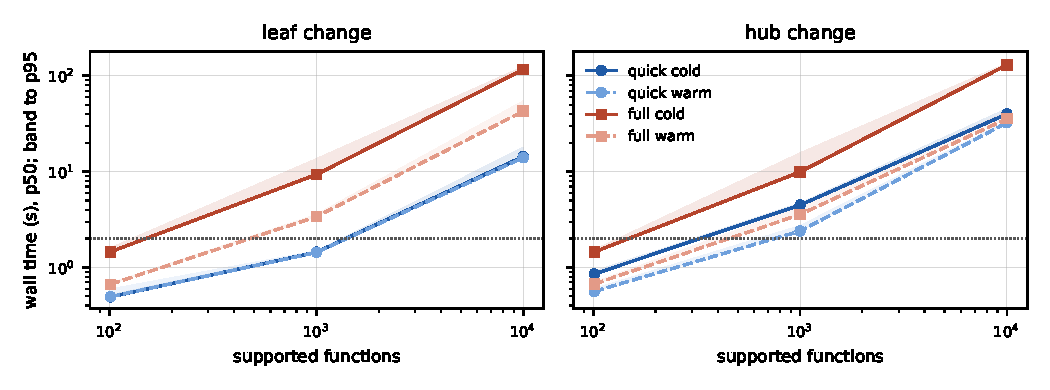
\includegraphics[width=\columnwidth]{generated/fig_latency.pdf}
\caption{Wall time of \texttt{guard verify} versus repository size (log-log; line = p50, band = p50 to p95). Dotted
line: the 2\,s default quick budget.}
\label{fig:latency}
\end{figure}

\begin{table*}[t]
\centering
\small

\caption{Incremental (quick, affected slice) versus full analysis at equal configuration: obligations of the quick report compared by ID with the full report. \emph{mismatch}: both make a claim and the claims differ; \emph{cov. loss}: quick is UNKNOWN (budget) where full decides; \emph{missed}: INTRODUCED findings of the full run absent from the quick run. \emph{callee}: a shared helper change that introduces real defects in unchanged callers.}
\label{tab:consistency}
\begin{tabular}{rlrrrrrrll}
\toprule
fns & change & compared & mismatch & cov. loss & intro.\textsubscript{full} & intro.\textsubscript{quick} & missed & verdict q/f & warm c/m/l \\
\midrule
101 & leaf & 3 & 0 & 0 & 0 & 0 & 0 & PASS/PASS & 3/0/0 \\
101 & hub & 61 & 0 & 0 & 0 & 0 & 0 & PASS/PASS & 61/0/0 \\
101 & callee & 48 & 0 & 0 & 21 & 21 & 0 & WARN/WARN & -- \\
1{,}001 & leaf & 3 & 0 & 0 & 0 & 0 & 0 & PASS/PASS & 3/0/0 \\
1{,}001 & hub & 722 & 0 & 64 & 0 & 0 & 0 & INCOMPLETE/PASS & 722/0/0 \\
1{,}001 & callee & 517 & 0 & 161 & 215 & 112 & 103 & INCOMPLETE/WARN & -- \\
10{,}001 & leaf & 3 & 0 & 0 & 0 & 0 & 0 & PASS/INCOMPLETE & 3/0/0 \\
10{,}001 & hub & 7{,}132 & 0 & 2{,}001 & 0 & 0 & 0 & INCOMPLETE/PASS & 7{,}132/0/2{,}001 \\
10{,}001 & callee & 4{,}721 & 0 & 3{,}079 & 1{,}928 & 0 & 1{,}928 & INCOMPLETE/WARN & -- \\
\bottomrule
\end{tabular}
\end{table*}


\subsection{RQ5: contract proposers}
\label{sec:rq5}

We compare three proposers on \ModelFunctions{} held-out functions. \ModelSeeded{} of them contain a seeded bug that
contradicts the function's own docstring; \SeededDslExpressible{} of these bugs are expressible in the DSL. Every candidate passed through the
same validation, non-vacuity, de-duplication and Docker falsification (32 probes). A refuted claim was then checked
against reference behavior: the intended reference implementation for seeded functions, the fixture itself otherwise.
It was checked at the counterexample and at 32 seeded inputs, which is a mechanical check, not a developer's review.
The proposers:
\begin{itemize}
\item \emph{Templates}: deterministic.
\item \emph{Local model}: \texttt{qwen2.5-coder:7b}, temperature~0, fixed seed, at most three candidates per function,
  \ModelRepeats{} repeats.
\item \emph{Agent-proposed}: \AgentRuns{} independent Claude Sonnet 5.5 subagents. Each saw only the \ModelFunctions{} context packets
  (identical to the model's packets) and the protocol README, and wrote up to eight candidates per function. The session
  transcripts show that no subagent read any other file or ran the tool. Scoring submitted the batches through the same
  code path as \texttt{guard contracts propose}, with templates in the same pass.
\end{itemize}

\begin{table*}[t]
\centering
\small

\caption{Contract proposers on the held-out set (13 functions, 5 seeded bugs), all through the same validation, non-vacuity filter, de-duplication and Docker falsification (32 probes). \emph{Templates}: deterministic, 3 repeats. \emph{Local model}: qwen2.5-coder:7b, temperature 0, at most 3 candidates per function, 3 repeats. \emph{Agent-proposed}: Claude Sonnet 5.5 subagents that saw only the context packets and the protocol README, at most 8 candidates per function, 3 independent runs; templates ran in the same pass so duplicates of template claims are excluded from \emph{new beyond templates}. Rates use each source's raw candidates as denominator. Wall time includes model inference (local model) or only validation and falsification (agent: proposals were written beforehand; each run took under two minutes by its session timestamps).}
\label{tab:model}
\begin{tabular}{llll}
\toprule
metric (one value per repeat) & templates & local model & agent-proposed \\
\midrule
raw candidates & 23, 23, 23 & 35, 35, 35 & 81, 89, 84 \\
schema-valid rate & 1.00, 1.00, 1.00 & 0.77, 0.77, 0.83 & 1.00, 1.00, 1.00 \\
non-vacuous rate & 1.00, 1.00, 1.00 & 0.66, 0.63, 0.69 & 1.00, 1.00, 1.00 \\
mech.\ checkable rate & 1.00, 1.00, 1.00 & 0.66, 0.63, 0.69 & 1.00, 1.00, 1.00 \\
distinct validated & 23, 23, 23 & 11, 9, 12 & 58, 66, 65 \\
\quad new beyond templates & -- & 11, 9, 12 & 58, 66, 65 \\
TESTED (distinct) & 23, 23, 23 & 1, 1, 2 & 52, 56, 56 \\
REFUTED (distinct) & 0, 0, 0 & 10, 8, 10 & 6, 10, 9 \\
\quad false claim & 0, 0, 0 & 8, 6, 8 & 0, 0, 0 \\
\quad valid for intent & 0, 0, 0 & 2, 2, 2 & 6, 10, 9 \\
seeded bugs exposed (of 5) & 0, 0, 0 & 2, 2, 2 & 5, 5, 5 \\
wall time (s) & 21, 21, 23 & 1071, 1398, 1174 & 85, 99, 83 \\
\bottomrule
\end{tabular}
\end{table*}


Table~\ref{tab:model} shows the results.
\begin{itemize}
\item \emph{Templates} produced \TemplateRawCands{} candidates per repeat, all \res{TESTED}, and exposed
  \TemplateExposed{} seeded bugs. They describe shape (purity, length, repeatability), not intent.
\item \emph{The local model} produced \ModelRawCands{} raw candidates and exposed \ModelExposed{} seeded bugs per repeat
  (\ModelExposedFns). \ModelFalseClaims{} of its claims per repeat were false about the intended behavior; they were
  refuted, so none would have been recorded. Its answers differed across repeats at temperature~0 with a fixed seed
  (\ModelDistinctResponseSets{} distinct response sets in \ModelRepeats{} repeats).
\item \emph{The agent} produced \AgentRawCands{} candidates per run, all schema-valid and non-vacuous, with no batch
  rejected. It exposed \AgentExposed{} of the \ModelSeeded{} seeded bugs per run (\AgentExposedFns), with
  \AgentFalseClaims{} false claims refuted per run. Bugs exposed in every agent run: \ExposedEveryAgentRun. Bugs exposed
  in every local-model repeat: \ExposedEveryModelRun. Bugs that only the agent exposed: \ExposedOnlyAgent.
\end{itemize}

This comparison is \emph{not} controlled, and four differences favor the agent:
\begin{itemize}
\item \emph{Different instructions.} The local model's system prompt asks it to ``claim only what the code or its
  documentation supports'' and to propose fewer candidates rather than guess. The agent harness additionally asked for
  ``properties that a maintainer would plausibly intend, including ones that might expose bugs''. The README the agents
  read describes the seeded-bug metric.
\item \emph{Different caps}: eight candidates per function versus three.
\item \emph{Model scale.} The agent is a much larger hosted model than a 7B quantized model running on the laptop.
\item \emph{Same family as the author.} The held-out functions, their docstrings and the DSL were written by a model of
  the same family (Section~\ref{sec:threats}).
\end{itemize}
The result therefore shows that the pipeline accepts agent proposals and that the same falsification filter applies to
them. It does not show that one proposer is better in general.

\paragraph{Cost.}
Model inference dominated the local arm: per function, \ModelLatPfifty\,s at p50 and \ModelLatPninetyfive\,s at p95,
over \ModelCalls{} answered calls; the inference server peaked at \ModelRss\,MB RSS. Discovery is therefore an explicit
command and never part of \texttt{guard verify}. By the session transcripts' timestamps, each agent run wrote its proposals in under two minutes; agent
token usage was not metered. Validating and falsifying them took \AgentFalsificationMin\,min per run.

\paragraph{Transport check.}
We also pointed the bring-your-own-key OpenAI-compatible adapter at the \emph{same} local Ollama server's \texttt{/v1}
endpoint for one pass over the \ModelFunctions{} functions. This checks transport, not quality. The adapter reported
\TransportStatus{}. All \TransportAnswered{} of \TransportFunctions{} functions were answered, with structured output
\TransportStructured{} and served model \TransportServed{}. The egress record states that context left the machine:
\TransportLeft. The pass produced \TransportRaw{} raw candidates at a schema-valid rate of \TransportSchemaRate{}, and
\TransportExposed{} seeded bugs were exposed, with a per-function latency of \TransportLatPfifty\,s at p50. We do not
treat these as a second quality estimate, for three reasons: it is the same model; it is a single pass; and the request
differs from the native arm (no digest pin, no explicit context size, \texttt{response\_format} instead of Ollama's
\texttt{format}). No hosted third-party provider was evaluated. The Anthropic adapter and hosted OpenAI-compatible
endpoints have been exercised only against local fakes in the test suite.

\section{Threats to validity}
\label{sec:threats}

\begin{itemize}
\item \emph{Author-written benchmarks, and an AI author.} The fixtures, the seeded patches, the held-out functions, the
  ground-truth oracle and the tool were all written by AI coding agents (Claude Opus 5.5) working from one
  specification. Those agents knew the supported subset. Labels were frozen before the tool ran, but case selection
  still reflects that knowledge. The seeded set is small (\SeedCases{} cases) and is not a sample of natural agent
  mistakes.
\item \emph{Same model family as the proposer.} The agent proposer (Claude Sonnet 5.5) comes from the same family as the
  model that wrote the held-out functions and their docstrings. It may share their idioms. It was blinded to everything
  except the context packets and the protocol README, but that README states that seeded bugs are scored. The prompts
  and candidate caps also differ between arms (Section~\ref{sec:rq5}).
\item \emph{Not held out.} The semantic fixtures were used as regression tests during development. One ground-truth
  field (the source line that a safe label refers to, for a function with two division sites) was added after a smoke
  run. No label changed.
\item \emph{One local model, one machine.} We evaluated one 7B quantized open-weight model on one laptop-class host
  under uncontrolled background load. Latency and model results may not transfer.
\item \emph{Ground truth.} Defect labels are confirmed by execution. Safe labels rest on hand arguments plus finite
  grids, which corroborate but do not prove. The check of whether a model claim is valid uses our own reference
  implementations and DSL evaluator.
\item \emph{Small counts.} Precision and recall over a few dozen cases have wide uncertainty. We report raw counts so that
  readers can compute their own intervals, and we report no per-finding probabilities.
\end{itemize}

\section{Related work}
\label{sec:related}

REDO~\cite{li2024redo} detects runtime errors in coding-agent patches without executing them, by combining static
analysis with an LLM. That is close to the goal of our static engine. We have not run REDO, and our benchmark is not
comparable to its benchmark. In agentic property-based testing~\cite{maaz2025agentic,anthropic2026pbt}, an agent infers
properties from code and documentation, tests them with Hypothesis~\cite{maciver2019hypothesis}, and reports bugs. Our
contract discovery overlaps with this work. Our version restricts every proposer, including a coding agent, to a typed
DSL whose candidates are falsified mechanically and carry no authority. Daikon~\cite{ernst2007daikon} and
DIG~\cite{nguyen2014dig,dig_repo} infer likely invariants from executions. Their observation that inferred invariants
describe observed behavior rather than intent motivates our separate authority axis. Z3~\cite{demoura2008z3} is our
solver, and agents consume our results over MCP~\cite{mcp2025transports}. We make no comparative performance claims
against any of these systems.

\section{Limitations}

\begin{itemize}
\item \emph{Narrow static subset.} It excludes loops, comprehensions, methods, closures, exception handlers and
  floating-point values. On realistic code many required obligations will be \res{UNKNOWN}, so honest verdicts will often
  be \res{INCOMPLETE}.
\item \emph{Quick mode.} It recomputes both snapshots in full and misses the latency target at scale. Its fingerprint
  defect (RQ4) can yield \res{PASS} for a change inside an unsupported nested function.
\item \emph{Finite contract evidence.} Contract checks give finite evidence over bounded built-in inputs only.
\item \emph{Coverage.} Only Python is implemented. The remote adapters have not been run against a hosted provider.
\item \emph{Agent repair.} The repository has one recorded agent repair loop. It is a single demonstration, not a rate,
  and its agent was a local-model harness, not a production coding agent.
\end{itemize}

\section{Conclusion}

Keeping proof, scope, authority, patch relation and coverage apart made the prototype's results checkable. In our
seeded set, every flagged defect carried either a validated witness or a replayed counterexample. Abstentions were
counted instead of hidden, and the same discipline exposed a real defect in the tool itself. Treating every proposer
(templates, a local model or a coding agent) as an untrusted source of typed, falsifiable candidates let three very
different proposers share one pipeline, with no candidate gaining authority. The evidence here is engineering evidence
on small synthetic benchmarks. Several questions remain open: effectiveness on natural agent patches, the value of
proposed contracts to developers, and performance at repository scale. Answering them requires held-out real-world
tasks, multiple independent models and authors, and human review.

{\small
\bibliographystyle{plainnat}
\bibliography{refs}
}

\onecolumn
\appendix
\section{Per-case and latency details}
The tables below are generated from the same results files as the main text.
\begin{table*}[h!]
\centering
\small

\caption{Seeded baseline/patch pairs, one row per case (labels frozen before any tool run; ``?'' = execution did not confirm the label). Predictions: F = flagged (an INTRODUCED/CHANGED failure finding), C = clear, A = abstained (required coverage missing); the verdict follows the slash. \emph{execute} adds dynamic contract checks in the Docker runner (cases with contracts only).}
\label{tab:seeded-cases}
\begin{tabular}{lllllll}
\toprule
ID & class & label & quick & no-solver & full & execute \\
\midrule
S01 & div. guard removed & defect & F/BLOCK & F & F/BLOCK & -- \\
S02 & div. expression changed & defect & F/BLOCK & F & F/BLOCK & -- \\
S03 & div. guard weakened & defect & F/BLOCK & F & F/BLOCK & -- \\
S04 & div. guard weakened & defect & F/WARN & F & F/WARN & -- \\
S05 & div. guard reordered & defect & F/BLOCK & F & F/BLOCK & -- \\
S06 & changed callee & defect & F/BLOCK & F & F/BLOCK & -- \\
S07 & changed callee & defect & F/WARN & F & F/WARN & -- \\
S08 & changed constant & defect & F/BLOCK & F & F/BLOCK & -- \\
S09 & index guard removed & defect & F/BLOCK & F & F/BLOCK & -- \\
S10 & index off by one & defect & F/BLOCK & F & F/BLOCK & -- \\
S11 & index off by one & defect & F/BLOCK & F & F/BLOCK & -- \\
S12 & None guard removed & defect & F/BLOCK & F & F/BLOCK & -- \\
S13 & None from callee & defect & F/BLOCK & F & F/BLOCK & -- \\
D01 & contract: normalization & defect & A/INCOMPLETE & A & A/INCOMPLETE & F/BLOCK \\
D02 & contract: purity & defect & C/PASS & C & C/PASS & F/BLOCK \\
D03 & contract: length & defect & C/PASS & C & C/PASS & F/BLOCK \\
D04 & contract: range & defect & C/PASS & C & C/PASS & F/BLOCK \\
D05 & contract + static div. & defect & A/INCOMPLETE & A & A/INCOMPLETE & F/BLOCK \\
I01 & intentional, revised & none & A/INCOMPLETE & A & A/INCOMPLETE & A/INCOMPLETE \\
I02 & intentional, inferred & intent. & C/PASS & C & C/PASS & F/WARN \\
I03 & intentional, static & none & C/PASS & C & C/PASS & -- \\
I04 & intentional, unrevised & intent. & A/INCOMPLETE & A & A/INCOMPLETE & F/BLOCK \\
N01 & safe refactor & none & C/PASS & C & C/PASS & -- \\
N02 & safe refactor & none & C/PASS & C & C/PASS & -- \\
N03 & safe refactor & none & C/PASS & C & C/PASS & -- \\
N04 & safe refactor & none & C/PASS & C & C/PASS & -- \\
N05 & safe refactor & none & C/PASS & C & C/PASS & -- \\
N06 & safe refactor (contract) & none & A/INCOMPLETE & A & A/INCOMPLETE & A/INCOMPLETE \\
N07 & safe refactor (contract) & none & C/PASS & C & C/PASS & C/PASS \\
U01 & unsupported: loop & defect & A/INCOMPLETE & A & A/INCOMPLETE & -- \\
U02 & unsupported: nested def & defect & C/PASS & C & A/INCOMPLETE & -- \\
U03 & unsupported: loop & none & A/INCOMPLETE & A & A/INCOMPLETE & -- \\
U04 & unsupported: ext. call & defect & A/INCOMPLETE & A & A/INCOMPLETE & -- \\
P01 & pre-existing (static) & none & A/INCOMPLETE & A & A/INCOMPLETE & -- \\
P02 & pre-existing (contract) & none & A/INCOMPLETE & A & A/INCOMPLETE & A/INCOMPLETE \\
\bottomrule
\end{tabular}
\end{table*}

\begin{table*}[h!]
\centering
\footnotesize
\setlength{\tabcolsep}{4pt}
\caption{Static \texttt{guard verify} latency on synthetic repositories (ms; fresh child process per run, interpreter start included). \emph{leaf}: one function body changes; \emph{hub}: a constant read by most functions changes. Default 2\,s quick budget. \emph{load}: median 1-minute load average sampled after each run (10 logical CPUs; values far above 10 mean heavy contention from other processes on the host).}
\label{tab:latency}
\begin{tabular}{rllllrrrrrlr}
\toprule
fns & change & mode & cache & n & wall p50 & wall p95 & engine p50 & RSS MB & affected & verdict (runs) & load \\
\midrule
101 & leaf & quick & cold & 30 & 493 & 517 & 156 & 39 & 2 & PASS & 7 \\
101 & leaf & quick & warm & 30 & 496 & 598 & 155 & 40 & 2 & PASS & 6 \\
101 & leaf & full & cold & 30 & 1{,}456 & 1{,}607 & 932 & 82 & 2 & PASS & 5 \\
101 & leaf & full & warm & 30 & 668 & 690 & 167 & 46 & 2 & PASS & 4 \\
101 & hub & quick & cold & 30 & 855 & 916 & 439 & 66 & 48 & PASS & 3 \\
101 & hub & quick & warm & 30 & 563 & 604 & 159 & 42 & 48 & PASS & 3 \\
101 & hub & full & cold & 30 & 1{,}450 & 1{,}536 & 927 & 81 & 48 & PASS & 3 \\
101 & hub & full & warm & 30 & 672 & 704 & 168 & 45 & 48 & PASS & 3 \\
1{,}001 & leaf & quick & cold & 30 & 1{,}445 & 1{,}488 & 1{,}016 & 84 & 2 & PASS & 2 \\
1{,}001 & leaf & quick & warm & 30 & 1{,}435 & 1{,}495 & 1{,}011 & 84 & 2 & PASS & 2 \\
1{,}001 & leaf & full & cold & 30 & 9{,}334 & 13{,}711 & 7{,}046 & 180 & 2 & PASS & 4 \\
1{,}001 & leaf & full & warm & 30 & 3{,}388 & 3{,}599 & 1{,}197 & 152 & 2 & PASS & 2 \\
1{,}001 & hub & quick & cold & 30 & 4{,}483 & 4{,}711 & 3{,}145 & 135 & 570 & INCOMPLETE & 4 \\
1{,}001 & hub & quick & warm & 30 & 2{,}401 & 2{,}741 & 1{,}116 & 118 & 570 & PASS & 5 \\
1{,}001 & hub & full & cold & 30 & 9{,}930 & 15{,}753 & 7{,}671 & 173 & 570 & PASS & 5 \\
1{,}001 & hub & full & warm & 30 & 3{,}578 & 4{,}293 & 1{,}260 & 152 & 570 & PASS & 7 \\
10{,}001 & leaf & quick & cold & 5 & 14{,}335 & 17{,}925 & 13{,}223 & 380 & 2 & PASS & 6 \\
10{,}001 & leaf & quick & warm & 5 & 13{,}961 & 14{,}307 & 12{,}851 & 375 & 2 & PASS & 6 \\
10{,}001 & leaf & full & cold & 5 & 116{,}354 & 124{,}784 & 91{,}375 & 549 & 2 & INCOMPLETE (2); PASS (3) & 6 \\
10{,}001 & leaf & full & warm & 5 & 42{,}714 & 54{,}785 & 18{,}945 & 599 & 2 & PASS & 5 \\
10{,}001 & hub & quick & cold & 5 & 39{,}896 & 45{,}567 & 27{,}315 & 492 & 5{,}749 & INCOMPLETE & 6 \\
10{,}001 & hub & quick & warm & 5 & 32{,}328 & 33{,}837 & 18{,}679 & 514 & 5{,}749 & INCOMPLETE & 6 \\
10{,}001 & hub & full & cold & 5 & 129{,}902 & 135{,}368 & 107{,}396 & 565 & 5{,}749 & PASS & 8 \\
10{,}001 & hub & full & warm & 5 & 35{,}696 & 42{,}447 & 17{,}783 & 698 & 5{,}749 & PASS & 5 \\
\bottomrule
\end{tabular}
\end{table*}

\begin{table*}[h!]
\centering
\small

\caption{Where cold \texttt{guard verify} time goes (p50 per phase, ms). \emph{capture}: reading and hashing the candidate snapshot (working tree); \emph{base capture}: the base commit (Git object reads); \emph{analysis}: lowering and static analysis of the candidate (solver time included); \emph{solver}: Z3 time alone; \emph{impact}: matching symbols and computing the slice. \emph{engine} is the sum of the report's timing fields excluding solver; \emph{wall} adds interpreter start, imports and report serialization/validation. No model is involved in any of these runs.}
\label{tab:phases}
\begin{tabular}{rllrrrrrrrr}
\toprule
fns & change & mode & capture & base capture & analysis & base analysis & solver & impact & engine & wall \\
\midrule
101 & leaf & quick & 31 & 29 & 46 & 47 & 0 & 3 & 156 & 493 \\
101 & leaf & full & 31 & 29 & 421 & 443 & 91 & 3 & 932 & 1{,}456 \\
101 & hub & quick & 31 & 29 & 181 & 190 & 26 & 3 & 439 & 855 \\
101 & hub & full & 31 & 29 & 425 & 437 & 91 & 3 & 927 & 1{,}450 \\
1{,}001 & leaf & quick & 35 & 34 & 487 & 429 & 0 & 31 & 1{,}016 & 1{,}445 \\
1{,}001 & leaf & full & 34 & 36 & 3{,}488 & 3{,}434 & 659 & 30 & 7{,}046 & 9{,}334 \\
1{,}001 & hub & quick & 35 & 34 & 1{,}366 & 1{,}665 & 136 & 31 & 3{,}145 & 4{,}483 \\
1{,}001 & hub & full & 37 & 38 & 3{,}704 & 3{,}803 & 699 & 32 & 7{,}671 & 9{,}930 \\
10{,}001 & leaf & quick & 75 & 116 & 7{,}329 & 5{,}476 & 0 & 337 & 13{,}223 & 14{,}335 \\
10{,}001 & leaf & full & 115 & 133 & 41{,}194 & 43{,}222 & 7{,}000 & 357 & 91{,}375 & 116{,}354 \\
10{,}001 & hub & quick & 117 & 151 & 13{,}227 & 13{,}508 & 0 & 605 & 27{,}315 & 39{,}896 \\
10{,}001 & hub & full & 129 & 152 & 56{,}804 & 50{,}899 & 8{,}813 & 367 & 107{,}396 & 129{,}902 \\
\bottomrule
\end{tabular}
\end{table*}

\begin{table*}[h!]
\centering
\footnotesize
\setlength{\tabcolsep}{4pt}
\caption{The two latency runs (DECISIONS I-111): the first run (pipeline order, with host load spikes) and the pre-registered repeat at the end of the pipeline, which the main text reports. Wall p50 in ms; \emph{load}: median 1-minute load average after each run (10 logical CPUs); \emph{ratio}: first / repeat. INC = INCOMPLETE: required obligations stayed UNKNOWN (in quick mode the 2\,s budget ran out; in full mode \LatFullUnresolvedMin--\LatFullUnresolvedMax{} obligations stayed UNKNOWN without the 600\,s budget being reached).}
\label{tab:latency-runs}
\begin{tabular}{rlllrrrlrrlr}
\toprule
fns & change & mode & cache & n & p50 first & load & verdict first & p50 repeat & load & verdict repeat & ratio \\
\midrule
101 & leaf & quick & cold & 30 & 498 & 7 & PASS & 493 & 7 & PASS & 1.01 \\
101 & leaf & quick & warm & 30 & 486 & 6 & PASS & 496 & 6 & PASS & 0.98 \\
101 & leaf & full & cold & 30 & 1{,}653 & 6 & PASS & 1{,}456 & 5 & PASS & 1.14 \\
101 & leaf & full & warm & 30 & 701 & 6 & PASS & 668 & 4 & PASS & 1.05 \\
101 & hub & quick & cold & 30 & 911 & 6 & PASS & 855 & 3 & PASS & 1.06 \\
101 & hub & quick & warm & 30 & 636 & 7 & PASS & 563 & 3 & PASS & 1.13 \\
101 & hub & full & cold & 30 & 1{,}645 & 6 & PASS & 1{,}450 & 3 & PASS & 1.13 \\
101 & hub & full & warm & 30 & 824 & 9 & PASS & 672 & 3 & PASS & 1.22 \\
1{,}001 & leaf & quick & cold & 30 & 1{,}498 & 11 & PASS & 1{,}445 & 2 & PASS & 1.04 \\
1{,}001 & leaf & quick & warm & 30 & 1{,}478 & 9 & PASS & 1{,}435 & 2 & PASS & 1.03 \\
1{,}001 & leaf & full & cold & 30 & 10{,}048 & 5 & PASS & 9{,}334 & 4 & PASS & 1.08 \\
1{,}001 & leaf & full & warm & 30 & 3{,}655 & 9 & PASS & 3{,}388 & 2 & PASS & 1.08 \\
1{,}001 & hub & quick & cold & 30 & 4{,}526 & 7 & INC & 4{,}483 & 4 & INC & 1.01 \\
1{,}001 & hub & quick & warm & 30 & 2{,}745 & 21 & PASS & 2{,}401 & 5 & PASS & 1.14 \\
1{,}001 & hub & full & cold & 30 & 27{,}684 & 36 & INC (7); PASS (23) & 9{,}930 & 5 & PASS & 2.79 \\
1{,}001 & hub & full & warm & 30 & 11{,}378 & 29 & PASS & 3{,}578 & 7 & PASS & 3.18 \\
10{,}001 & leaf & quick & cold & 5 & 59{,}690 & 31 & PASS & 14{,}335 & 6 & PASS & 4.16 \\
10{,}001 & leaf & quick & warm & 5 & 16{,}179 & 20 & PASS & 13{,}961 & 6 & PASS & 1.16 \\
10{,}001 & leaf & full & cold & 5 & 133{,}850 & 8 & INC (1); PASS (4) & 116{,}354 & 6 & INC (2); PASS (3) & 1.15 \\
10{,}001 & leaf & full & warm & 5 & 38{,}258 & 5 & PASS & 42{,}714 & 5 & PASS & 0.90 \\
10{,}001 & hub & quick & cold & 5 & 34{,}733 & 4 & INC & 39{,}896 & 6 & INC & 0.87 \\
10{,}001 & hub & quick & warm & 5 & 33{,}342 & 8 & INC & 32{,}328 & 6 & INC & 1.03 \\
10{,}001 & hub & full & cold & 5 & 118{,}210 & 6 & PASS & 129{,}902 & 8 & PASS & 0.91 \\
10{,}001 & hub & full & warm & 5 & 34{,}941 & 8 & PASS & 35{,}696 & 5 & PASS & 0.98 \\
\bottomrule
\end{tabular}
\end{table*}


\end{document}
